\documentclass[]{elsarticle} %review=doublespace preprint=single 5p=2 column
%%% Begin My package additions %%%%%%%%%%%%%%%%%%%
\usepackage[hyphens]{url}

  \journal{TBD} % Sets Journal name


\usepackage{lineno} % add
\providecommand{\tightlist}{%
  \setlength{\itemsep}{0pt}\setlength{\parskip}{0pt}}

\usepackage{graphicx}
%%%%%%%%%%%%%%%% end my additions to header

\usepackage[T1]{fontenc}
\usepackage{lmodern}
\usepackage{amssymb,amsmath}
\usepackage{ifxetex,ifluatex}
\usepackage{fixltx2e} % provides \textsubscript
% use upquote if available, for straight quotes in verbatim environments
\IfFileExists{upquote.sty}{\usepackage{upquote}}{}
\ifnum 0\ifxetex 1\fi\ifluatex 1\fi=0 % if pdftex
  \usepackage[utf8]{inputenc}
\else % if luatex or xelatex
  \usepackage{fontspec}
  \ifxetex
    \usepackage{xltxtra,xunicode}
  \fi
  \defaultfontfeatures{Mapping=tex-text,Scale=MatchLowercase}
  \newcommand{\euro}{€}
\fi
% use microtype if available
\IfFileExists{microtype.sty}{\usepackage{microtype}}{}
\bibliographystyle{elsarticle-harv}
\usepackage{longtable,booktabs,array}
\usepackage{calc} % for calculating minipage widths
% Correct order of tables after \paragraph or \subparagraph
\usepackage{etoolbox}
\makeatletter
\patchcmd\longtable{\par}{\if@noskipsec\mbox{}\fi\par}{}{}
\makeatother
% Allow footnotes in longtable head/foot
\IfFileExists{footnotehyper.sty}{\usepackage{footnotehyper}}{\usepackage{footnote}}
\makesavenoteenv{longtable}
\ifxetex
  \usepackage[setpagesize=false, % page size defined by xetex
              unicode=false, % unicode breaks when used with xetex
              xetex]{hyperref}
\else
  \usepackage[unicode=true]{hyperref}
\fi
\hypersetup{breaklinks=true,
            bookmarks=true,
            pdfauthor={},
            pdftitle={Influence of School Closure on COVID-19 Contaminations in Ireland and Repercussions across Age Groups},
            colorlinks=false,
            urlcolor=blue,
            linkcolor=magenta,
            pdfborder={0 0 0}}
\urlstyle{same}  % don't use monospace font for urls

\setcounter{secnumdepth}{5}
% Pandoc toggle for numbering sections (defaults to be off)

% Pandoc citation processing
\newlength{\cslhangindent}
\setlength{\cslhangindent}{1.5em}
\newlength{\csllabelwidth}
\setlength{\csllabelwidth}{3em}
% for Pandoc 2.8 to 2.10.1
\newenvironment{cslreferences}%
  {}%
  {\par}
% For Pandoc 2.11+
\newenvironment{CSLReferences}[2] % #1 hanging-ident, #2 entry spacing
 {% don't indent paragraphs
  \setlength{\parindent}{0pt}
  % turn on hanging indent if param 1 is 1
  \ifodd #1 \everypar{\setlength{\hangindent}{\cslhangindent}}\ignorespaces\fi
  % set entry spacing
  \ifnum #2 > 0
  \setlength{\parskip}{#2\baselineskip}
  \fi
 }%
 {}
\usepackage{calc}
\newcommand{\CSLBlock}[1]{#1\hfill\break}
\newcommand{\CSLLeftMargin}[1]{\parbox[t]{\csllabelwidth}{#1}}
\newcommand{\CSLRightInline}[1]{\parbox[t]{\linewidth - \csllabelwidth}{#1}\break}
\newcommand{\CSLIndent}[1]{\hspace{\cslhangindent}#1}

% Pandoc header
\usepackage{booktabs}
\usepackage{float}



\begin{document}
\begin{frontmatter}

  \title{Influence of School Closure on COVID-19 Contaminations in Ireland and Repercussions across Age Groups}
    \author[Dublin City University]{Edgar Morgenroth\corref{1}}
   \ead{edgar.morgenroth@dcu.ie} 
    \author[Dublin City University]{Damien Dupré\corref{2}}
   \ead{damien.dupre@dcu.ie} 
      \address[Dublin City University]{Glasnevin, Dublin 9, Ireland}
      \cortext[1]{Corresponding Author}
    \cortext[2]{Equal contribution}
  
  \begin{abstract}
  TBD
  \end{abstract}
  
 \end{frontmatter}




\hypertarget{introduction}{%
\section{Introduction}\label{introduction}}

Since the onset of Covid-19, contradicting messages are circulating about the spread of the virus in schools. Sometimes presented as a safe environment (Falk et al., 2021; Walger et al., 2020), at other times designed as an aggravating factor of the pandemic (Lopez et al., 2020; Meuris et al., 2021), child care facilities and schools have been closed multiple times in most countries to protect the public health. However, the efficacy of school closure is still unknown and little is know about how Covid-19 Cases spread across age cohort and especially from the younger cohort being at school to older cohorts including parents, grand parents and relatives. Some evidence show that school is an influential environment where the virus is likely to spread. Once contaminated at school, a common spread believe is that the children and teenagers will then contaminate their parents. Therefore, among the political actions to stop the spread of Covid-19, the closure of primary and secondary schools was widely adopted worldwide. This research aims to investigate 1) the effect of school closure on the evolution of Covid-19 cases and 2) the temporal relationship between the rise of cases in children and teenagers with the rise of cases of older age group.

\hypertarget{influence-of-school-closure}{%
\subsection{Influence of School Closure}\label{influence-of-school-closure}}

One of the strongest assumption of government actions is that by reducing social contact will reduce the spread of the virus. Therefore, it is legitimate to believe that by closing schools, a reduction of the contaminations would be observed in the younger age groups. However, the efficiency of school closure on the reduction of Covid-19 cases is still questioned. While some research have observed that school closures contribute to limit or to reduce the growth rate of confirmed cases after implementation (Stage et al., 2021; Sugishita, 2020), other did not observe a change in the evolution of Covid-19 cases (Chang et al., 2020; Iwata et al., 2020). For instance, a controlled comparison between similar localities in Japan with schools closed and school open did not revealed any evidence that school closures reduced the spread of Covid-19 (Fukumoto et al., 2021). If the school closure had a real impact on the evolution of confirmed Covid-19 cases, it should be possible to observe a decrease or a least an inflection in the trend of its evolution among younger age groups.

\hypertarget{causal-relationship-between-age-groups}{%
\subsection{Causal Relationship Between Age Groups}\label{causal-relationship-between-age-groups}}

A second implicit believe regarding the effect of school closure on the spread of Covid-19 is that school not only has an effect on to the spread of the virus in children and teenagers but also has a knock-on effect on the spread of the virus in older age groups also called Secondary Attack Rate (SAR). The contaminated children and teenagers would bring the virus back at home and, then, they will contaminate their parents and relatives. For example, a research investigating the contamination in the household network not only revealed an exceptional high rate of secondary contamination but also that these contamination happened when the school were closed (Soriano-Arandes et al., 2021).

Despite being reported in several clinical and epidemiological studies (Siebach et al., 2021; Zhen-Dong et al., 2020), multiple research have shown that the SAR from children to household members was, in fact, lower than expected (Heavey et al., 2020; Hoek et al., 2020; Kim et al., 2021; Ludvigsson, 2020). However, the SAR of children and teenagers to the household member is likely to be age-dependent, with difference between infants, primary and secondary school children, and college students (Gras-Le Guen et al., 2021). If a secondary transmission from children and teenagers to household member has a significant influence, then a temporal causality relationship between their evolution should be observed.

\hypertarget{method}{%
\section{Method}\label{method}}

\hypertarget{observations}{%
\subsection{Observations}\label{observations}}

The data were collected from the official daily publication of Covid-19 cases by the Irish Department of Health. They include the amount of daily cases for 10 age groups from March 04, 2020 to January 01, 2022. For each day during this period, school closure either due to a government decision or a public holiday is determined.

\hypertarget{data-pre-processing}{%
\subsection{Data Pre-processing}\label{data-pre-processing}}

A 7-day rolling average of the day-by-by change in Covid-19 cases reported (i.e., lag 1) is used to evaluate the efficiency of school closures. This rolling average approximate the real day-by-by change in Covid-19 cases reported which can be artificially increased or decreased due to days under- or over-reporting cases such as weekend or bank holidays for example.

\hypertarget{data-analysis}{%
\subsection{Data Analysis}\label{data-analysis}}

\hypertarget{generalised-additive-model}{%
\subsubsection{Generalised Additive Model}\label{generalised-additive-model}}

Four periods of school closure longer that 14 days have been identified. These four periods are used to fit a Generalised Additive Model (or GAM) using the R package mgcv (Wood, 2017) in order to test the hypothesis of a significant change in the evolution of cases among age groups from 1 to 4, from 5 to 14, and from 15 to 24.

By estimating the degree of smoothness of a Bayesian spline smoothing using restricted maximum likelihood estimation (Wood, 2011), GAM identifies dynamic patterns underlying the day-by-day changes in Covid-19 cases reported while taking into account the random effect of different age groups as follows:

\begin{align}
Y_{is} = \alpha_{i} + f(X_{s}) + a_{is} + \epsilon_{is}
\end{align}

\noindent where \(i\) is an age group among the 10 age groups investigated and \(s\) is the date corresponding to the day-by-day change in Covid-19 cases. \(Y_{is}\) represents the day-by-day change in Covid-19 cases assuming a negative binomial distribution for the fitting (Loader, 2006). The response variable \(Y_{is}\) includes a specific intercept for each age group (\(\alpha_{i}\)). A smooth effect over time \(f(X_{s})\) is applied to model (Eq 1) to predict the nonlinear evolution of day-by-day change in Covid-19 cases. This smooth effect \(f(X_{s})\) is built up in basic components, called the basis functions \(b_{j}(X_{s})\), such that:

\begin{align}
f(X_{s})=\sum_{j=1}^{k}\beta_{j}\times b_{j}(X_{s})
\end{align}

\noindent where the regression parameters \(\beta_{j}\) are estimated by penalized likelihood maximization.

The model also includes the random effects term \(a_{is}= Zb_{i}\) where \(Z\) is a random effects matrix and \(b_{i}\) is a vector of random effects described by \(b_{i} \sim N(0, D)\). In this, \(D\) represents a covariance matrix. The error term \(\epsilon_{is}\) is assumed to be normally and independently distributed \(\epsilon_{is} \sim N(0, \sigma^2)\).

\hypertarget{transfer-entropy}{%
\subsubsection{Transfer Entropy}\label{transfer-entropy}}

Transfer Entropy can be used to infer the temporal relationship between two time series \(I\) and \(J\). This measure indicates whether \(J\) can be used to to reduce the uncertainty on the future of \(I\) and, consequently, that \(J\) causes \(I\) (Schreiber, 2000). Contrary to Wiener-Granger Causality, Transfer Entropy is robust to non-stationary time series (Papana et al., 2016; Wollstadt, 2014). The Transfer Entropy analysis of younger age groups daily changes in Covid-19 cases on older age groups using Shannon's calculation (Shannon, 1948) is done using the R package RTransferEntropy (Behrendt et al., 2019).

The influence of day-by-day changes in Covid-19 cases across all age groups is evaluated using Shannon's transfer entropy is given by:

\begin{align}
  T_{J \rightarrow I}(k,l) = \sum_{i,j} p\left(i_{t+1}, i_t^{(k)}, j_t^{(l)}\right) \cdot log \left(\frac{p\left(i_{t+1}| i_t^{(k)}, j_t^{(l)}\right)}{p\left(i_{t+1}|i_t^{(k)}\right)}\right),
\end{align}

\noindent where \(T_{J\rightarrow I}\) consequently measures the influence of the change dynamic from an eage group \(J\) to another age group \(I\).

\hypertarget{results}{%
\section{Results}\label{results}}

Overall, the trend of comfirm Covid-19 cases in Ireland is similar to those of other European countries (Figure \ref{fig:overall}). Indeed it is possible to observe a significant increase corresponding to each of the 4 waves of transmission (March-April 2020, December 2020-January 2021, September-October 2021 and November-December 2021).

\begin{figure}[!h]
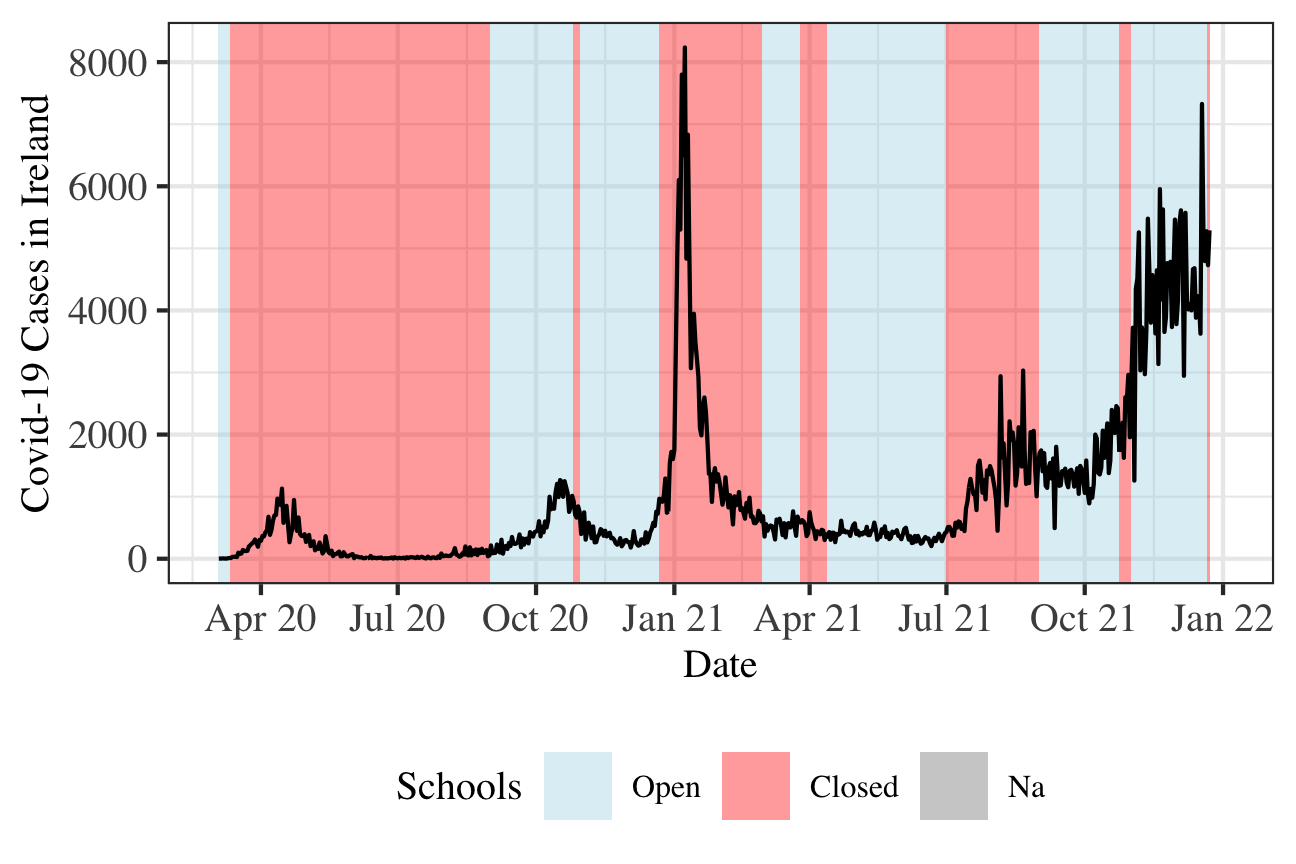
\includegraphics[width=324px]{/Users/damiendcu/OneDrive/Projects/covid_ts_causality/output/manuscript_2022-01-14_files/figure-latex/overall-1} \caption{Evolution of confirmed Covid-19 cases in Ireland alongside with school closures.}\label{fig:overall}
\end{figure}

The evolution of day-by-day changes in Covid-19 cases reveals some similarities across all age groups. However, the influence of each waves on the each groups has also some particularities (Figure \ref{fig:descriptive}). For example, the first wave was more important among the oldest age groups whereas the third wave was more important among the youngest age groups.

\begin{figure}
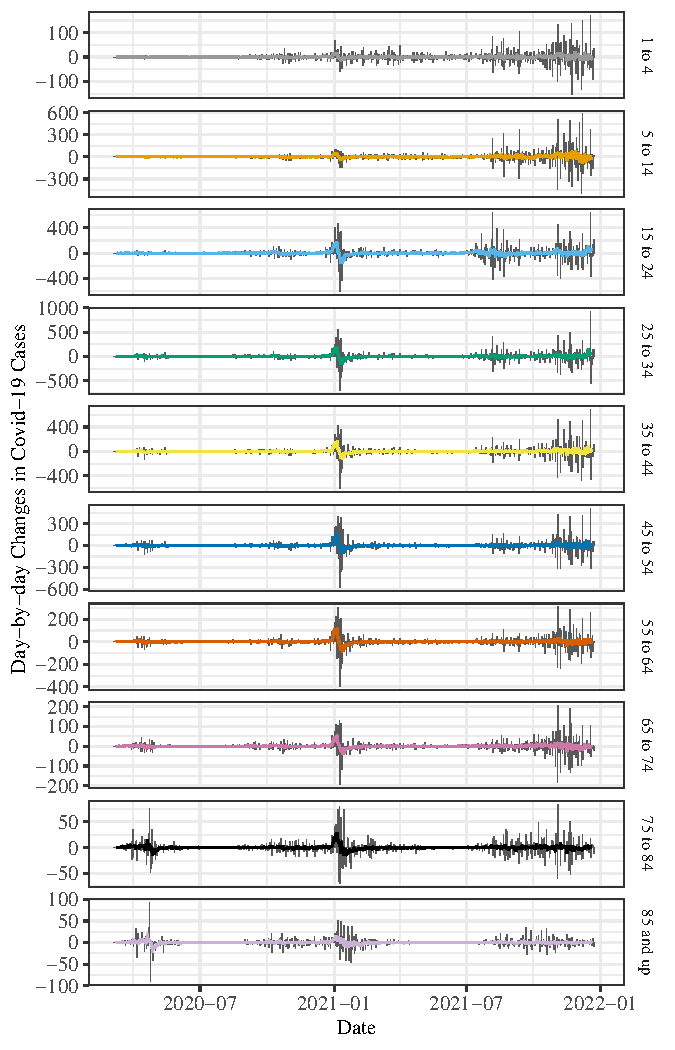
\includegraphics[width=324px]{/Users/damiendcu/OneDrive/Projects/covid_ts_causality/output/manuscript_2022-01-14_files/figure-latex/descriptive-1} \caption{Day-by-day changes in Covid-19 cases by age groups in Ireland: raw data (bars) and 7 aay rolling average (lines).}\label{fig:descriptive}
\end{figure}

\hypertarget{discussion}{%
\section{Discussion}\label{discussion}}

Knowledge about the transmission of the virus significantly improved with the amount of studies performed, especially in the case of how the virus behaves with children. From the early analyses showing that the virus was instantness in children (Li et al., 2020), the results has changed to more nuanced position which states that the spread of the virus in children is moderate.

\hypertarget{conclusion}{%
\section{Conclusion}\label{conclusion}}

\hypertarget{references}{%
\section*{References}\label{references}}
\addcontentsline{toc}{section}{References}

\hypertarget{refs}{}
\begin{CSLReferences}{1}{0}
\leavevmode\hypertarget{ref-behrendt2019rtransferentropy}{}%
Behrendt, S., Dimpfl, T., Peter, F.J., Zimmermann, D.J., 2019. RTransferEntropy --- quantifying information flow between different time series using effective transfer entropy. SoftwareX 10, 100265. doi:\href{https://doi.org/10.1016/j.softx.2019.100265}{10.1016/j.softx.2019.100265}

\leavevmode\hypertarget{ref-chang2020modelling}{}%
Chang, S.L., Harding, N., Zachreson, C., Cliff, O.M., Prokopenko, M., 2020. Modelling transmission and control of the COVID-19 pandemic in australia. Nature communications 11, 1--13. doi:\href{https://doi.org/10.1038/s41467-020-19393-6}{10.1038/s41467-020-19393-6}

\leavevmode\hypertarget{ref-falk2021covid}{}%
Falk, A., Benda, A., Falk, P., Steffen, S., Wallace, Z., Høeg, T.B., 2021. COVID-19 cases and transmission in 17 k--12 schools---wood county, wisconsin, august 31--november 29, 2020. Morbidity and Mortality Weekly Report 70, 136--140. doi:\href{https://doi.org/10.15585/mmwr.mm7004e3}{10.15585/mmwr.mm7004e3}

\leavevmode\hypertarget{ref-fukumoto2021no}{}%
Fukumoto, K., McClean, C.T., Nakagawa, K., 2021. No causal effect of school closures in japan on the spread of COVID-19 in spring 2020. Nature medicine 27, 2111--2119. doi:\href{https://doi.org/10.1038/s41591-021-01571-8}{10.1038/s41591-021-01571-8}

\leavevmode\hypertarget{ref-grasleguen2021reopening}{}%
Gras-Le Guen, C., Cohen, R., Rozenberg, J., Launay, E., Levy-Bruhl, D., Delacourt, C., 2021. Reopening schools in the context of increasing COVID-19 community transmission: The french experience. Archives de Pédiatrie 28, 178--185. doi:\href{https://doi.org/10.1016/j.arcped.2021.02.001}{10.1016/j.arcped.2021.02.001}

\leavevmode\hypertarget{ref-heavey2020evidence}{}%
Heavey, L., Casey, G., Kelly, C., Kelly, D., McDarby, G., 2020. No evidence of secondary transmission of COVID-19 from children attending school in ireland, 2020. Eurosurveillance 25. doi:\href{https://doi.org/10.2807/1560-7917.ES.2020.25.21.2000903}{10.2807/1560-7917.ES.2020.25.21.2000903}

\leavevmode\hypertarget{ref-vanderhoek2020role}{}%
Hoek, W. van der, Backer, J.A., Bodewes, R., Friesema, I., Meijer, A., Pijnacker, R., Reukers, D.F.M., Reusken, C., Roof, I., Rots, N., Te Wierik, M.J.M., Gageldonk-Lafeber, A. van, Waegemaekers, C., Hof, S. van den, 2020. The role of children in the transmission of SARS-CoV-2. Nederlands tijdschrift voor geneeskunde 164.

\leavevmode\hypertarget{ref-iwata2020school}{}%
Iwata, K., Doi, A., Miyakoshi, C., 2020. Was school closure effective in mitigating coronavirus disease 2019 (COVID-19)? Time series analysis using bayesian inference. International Journal of Infectious Diseases 99, 57--61. doi:\href{https://doi.org/10.1016/j.ijid.2020.07.052}{10.1016/j.ijid.2020.07.052}

\leavevmode\hypertarget{ref-kim2021role}{}%
Kim, J., Choe, Y.J., Lee, J., Park, Y.J., Park, O., Han, M.S., Kim, J.-H., Choi, E.H., 2021. Role of children in household transmission of COVID-19. Archives of Disease in Childhood 106, 709--711. doi:\href{https://doi.org/10.1136/archdischild-2020-319910}{10.1136/archdischild-2020-319910}

\leavevmode\hypertarget{ref-li2020role}{}%
Li, X., Xu, W., Dozier, M., He, Y., Kirolos, A., Theodoratou, E., others, 2020. The role of children in transmission of SARS-CoV-2: A rapid review. Journal of global health 10. doi:\href{https://doi.org/10.7189/jogh.10.011101}{10.7189/jogh.10.011101}

\leavevmode\hypertarget{ref-loader2006local}{}%
Loader, C., 2006. Local regression and likelihood. Springer, Boston, MA.

\leavevmode\hypertarget{ref-lopez2020transmission}{}%
Lopez, A.S., Hill, M., Antezano, J., Vilven, D., Rutner, T., Bogdanow, L., Claflin, C., Kracalik, I.T., Fields, V.L., Dunn, A., others, 2020. Transmission dynamics of COVID-19 outbreaks associated with child care facilities---salt lake city, utah, april--july 2020. Morbidity and Mortality Weekly Report 69, 1319. doi:\href{https://doi.org/10.15585/mmwr.mm6937e3}{10.15585/mmwr.mm6937e3}

\leavevmode\hypertarget{ref-ludvigsson2020children}{}%
Ludvigsson, J.F., 2020. Children are unlikely to be the main drivers of the COVID-19 pandemic -- a systematic review. Acta Paediatrica 109, 1525--1530. doi:\url{https://doi.org/10.1111/apa.15371}

\leavevmode\hypertarget{ref-meuris2021transmission}{}%
Meuris, C., Kremer, C., Geerinck, A., Locquet, M., Bruyère, O., Defêche, J., Meex, C., Hayette, M.-P., Duchene, L., Dellot, P., Azarzar, S., Maréchal, N., Sauvage, A.-S., Frippiat, F., Giot, J.-B., Léonard, P., Fombellida, K., Moutschen, M., Durkin, K., Artesi, M., Bours, V., Faes, C., Hens, N., Darcis, G., 2021. Transmission of SARS-CoV-2 after COVID-19 screening and mitigation measures for primary school children attending school in liège, belgium. JAMA Network Open 4, e2128757--e2128757. doi:\href{https://doi.org/10.1001/jamanetworkopen.2021.28757}{10.1001/jamanetworkopen.2021.28757}

\leavevmode\hypertarget{ref-papana2016detecting}{}%
Papana, A., Kyrtsou, C., Kugiumtzis, D., Diks, C., 2016. Detecting causality in non-stationary time series using partial symbolic transfer entropy: Evidence in financial data. Computational economics 47, 341--365. doi:\href{https://doi.org/10.1007/s10614-015-9491-x}{10.1007/s10614-015-9491-x}

\leavevmode\hypertarget{ref-schreiber2000measuring}{}%
Schreiber, T., 2000. Measuring information transfer. Phys. Rev. Lett. 85, 461--464. doi:\href{https://doi.org/10.1103/PhysRevLett.85.461}{10.1103/PhysRevLett.85.461}

\leavevmode\hypertarget{ref-shannon1948mathematical}{}%
Shannon, C.E., 1948. A mathematical theory of communication. The Bell system technical journal 27, 379--423.

\leavevmode\hypertarget{ref-siebach2021childhood}{}%
Siebach, M.K., Piedimonte, G., Ley, S.H., 2021. COVID-19 in childhood: Transmission, clinical presentation, complications and risk factors. Pediatric Pulmonology 56, 1342--1356. doi:\url{https://doi.org/10.1002/ppul.25344}

\leavevmode\hypertarget{ref-sorianoarandes2021household}{}%
Soriano-Arandes, A., Gatell, A., Serrano, P., Biosca, M., Campillo, F., Capdevila, R., Fàbrega, A., Lobato, Z., López, N., Moreno, A.M., Poblet, M., Riera-Bosch, M.T., Rius, N., Ruiz, M., Sánchez, A., Valldepérez, C., Vilà, M., Pineda, V., Lazcano, U., Díaz, Y., Reyes-Urueña, J., Soler-Palacín, P., Catalonia Research Group, C.P.D. in, 2021. Household severe acute respiratory syndrome coronavirus 2 transmission and children: A network prospective study. Clinical Infectious Diseases 73, e1261--e1269. doi:\href{https://doi.org/10.1093/cid/ciab228}{10.1093/cid/ciab228}

\leavevmode\hypertarget{ref-stage2021shut}{}%
Stage, H.B., Shingleton, J., Ghosh, S., Scarabel, F., Pellis, L., Finnie, T., 2021. Shut and re-open: The role of schools in the spread of COVID-19 in europe. Philosophical Transactions of the Royal Society B 376, 20200277. doi:\href{https://doi.org/10.1098/rstb.2020.0277}{10.1098/rstb.2020.0277}

\leavevmode\hypertarget{ref-yoshiyuki2020effects}{}%
Sugishita, J.A.S., Yoshiyuki AND Kurita, 2020. Effects of voluntary event cancellation and school closure as countermeasures against COVID-19 outbreak in japan. PLOS ONE 15, 1--10. doi:\href{https://doi.org/10.1371/journal.pone.0239455}{10.1371/journal.pone.0239455}

\leavevmode\hypertarget{ref-walger2020children}{}%
Walger, P., Heininger, U., Knuf, M., Exner, M., Popp, W., Fischbach, T., Trapp, S., Hübner, J., Herr, C., Simon, A., others, 2020. Children and adolescents in the CoVid-19 pandemic: Schools and daycare centers are to be opened again without restrictions. The protection of teachers, educators, carers and parents and the general hygiene rules do not conflict with this. GMS hygiene and infection control 15. doi:\href{https://doi.org/10.3205/dgkh000346}{10.3205/dgkh000346}

\leavevmode\hypertarget{ref-wollstadt2014efficient}{}%
Wollstadt, M.A.V., Patricia AND Martínez-Zarzuela, 2014. Efficient transfer entropy analysis of non-stationary neural time series. PLOS ONE 9, 1--21. doi:\href{https://doi.org/10.1371/journal.pone.0102833}{10.1371/journal.pone.0102833}

\leavevmode\hypertarget{ref-wood2011fast}{}%
Wood, S.N., 2011. Fast stable restricted maximum likelihood and marginal likelihood estimation of semiparametric generalized linear models. Journal of the Royal Statistical Society (B) 73, 3--36.

\leavevmode\hypertarget{ref-wood2017generalized}{}%
Wood, S.N., 2017. Generalized additive models: An introduction with r. CRC press.

\leavevmode\hypertarget{ref-zhendong2020clinical}{}%
Zhen-Dong, Y., Gao-Jun, Z., Run-Ming, J., Zhi-Sheng, L., Zong-Qi, D., Xiong, X., Guo-Wei, S., 2020. Clinical and transmission dynamics characteristics of 406 children with coronavirus disease 2019 in china: A review. Journal of Infection 81, e11--e15. doi:\href{https://doi.org/10.1016/j.jinf.2020.04.030}{10.1016/j.jinf.2020.04.030}

\end{CSLReferences}


\end{document}
